% !TEX root = ../proposal.tex

%\subsection{S/T Methodology and Associated Work Plan}
\subsection{Work plan -- Work packages, deliverables and milestones}

% Please provide the following:
%   - brief presentation of the overall structure of the work plan;
%   - timing of the different work packages and their components (Gantt
%     chart or similar);
%   - detailed work description, i.e.:
%     * a description of each work package (table 3.1a);
%     * a list of work packages (table 3.1b);
%     * a list of major deliverables (table 3.1c);
%   - graphical presentation of the components showing how they
%     inter-relate (Pert chart or similar).
%
% Give full details. Base your account on the logical structure of the
% project and the stages in which it is to be carried out. Include
% details of the resources to be allocated to each work package. The
% number of work packages should be proportionate to the scale and
% complexity of the project. 
%
% You should give enough detail in each work package to justify the
% proposed resources to be allocated and also quantified information so
% that progress can be monitored, including by the Commission. 
%
% You are advised to include a distinct work package on ‘management’
% (see section 3.2) and to give due visibility in the work plan to
% ‘dissemination and exploitation’ and ‘communication activities’,
% either with distinct tasks or distinct work packages.
%
% You will be required to include an updated (or confirmed) ‘plan for
% the dissemination and exploitation of results’ in both the periodic
% and final reports. (This does not apply to topics where a draft plan
% was not required.) This should include a record of activities related
% to dissemination and exploitation that have been undertaken and those
% still planned. A report of completed and planned communication
% activities will also be required.
%
% If your project is taking part in the Pilot on Open Research Data1,
% you must include a  'data management plan' as a distinct deliverable
% within the first 6 months of the project. A template for such a plan
% is given in the guidelines on data management in the H2020 Online
% Manual.  This deliverable will evolve during the lifetime of the
% project in order to present the status of the project's reflections on
% data management.
%
% Definitions: 
%  - ‘Work package’ means a major sub-division of the proposed project.
%  - ‘Deliverable’ means a distinct output of the project, meaningful in
%    terms of the project's overall objectives and constituted by a
%    report, a document, a technical diagram, a software etc.
%  - ‘Milestones’ means control points in the project that help to chart
%    progress. Milestones may correspond to the completion of a key
%    deliverable, allowing the next phase of the work to begin. They may
%    also be needed at intermediary points so that, if problems have
%    arisen, corrective measures can be taken. A milestone may be a
%    critical decision point in the project where, for example, the
%    consortium must decide which of several technologies to adopt for
%    further development.


\subsubsection{Overall Methodology}
\label{sec:workoverview}

\paragraph{\textbf{Iterative Life-Cycle Model}}

The technological aspects that will be developed by the \Project{} project represent step changes in TRL with respect to state of the art capabilities. As a result there is a need for a certain amount of experimentation with new functionality as well as significant iterative testing and validation during the development. Owing to this we plan to employ a \emph{spiral life-cycle model} within this project.

As illustrated in Figure~\ref{fig:spiral}, the spiral life-cycle model supports an iterative process comprised of the following phases: specification, research \& development, and integration \& evaluation. During the specification phase, initial requirements are gathered.  During the research and development phase, new basic research questions are proposed based upon the requirements derived during the specification phase.  This is then followed by the design and development of an evaluation platform that realizes these ideas.  During the integration and evaluation phase, the evaluation platform is then evaluated and further enhanced in the next iteration based on feedback.  The test results provide a new set of requirements, through redefining or completing the old set. With the second set of requirements, a new design and development cycle is performed that eliminates previous problems, and culminating in another evaluation.  That process is repeated until a complete set of functions meeting all requirements has been implemented.  Note that the specification, research \& development, as well as the evaluation phases typically show a certain level of concurrency and small overlaps during one cycle of the spiral.  In \Project{} the consortium will realize two cycles over the project duration.

\begin{wrapfigure}{r}{0.6\textwidth}%
    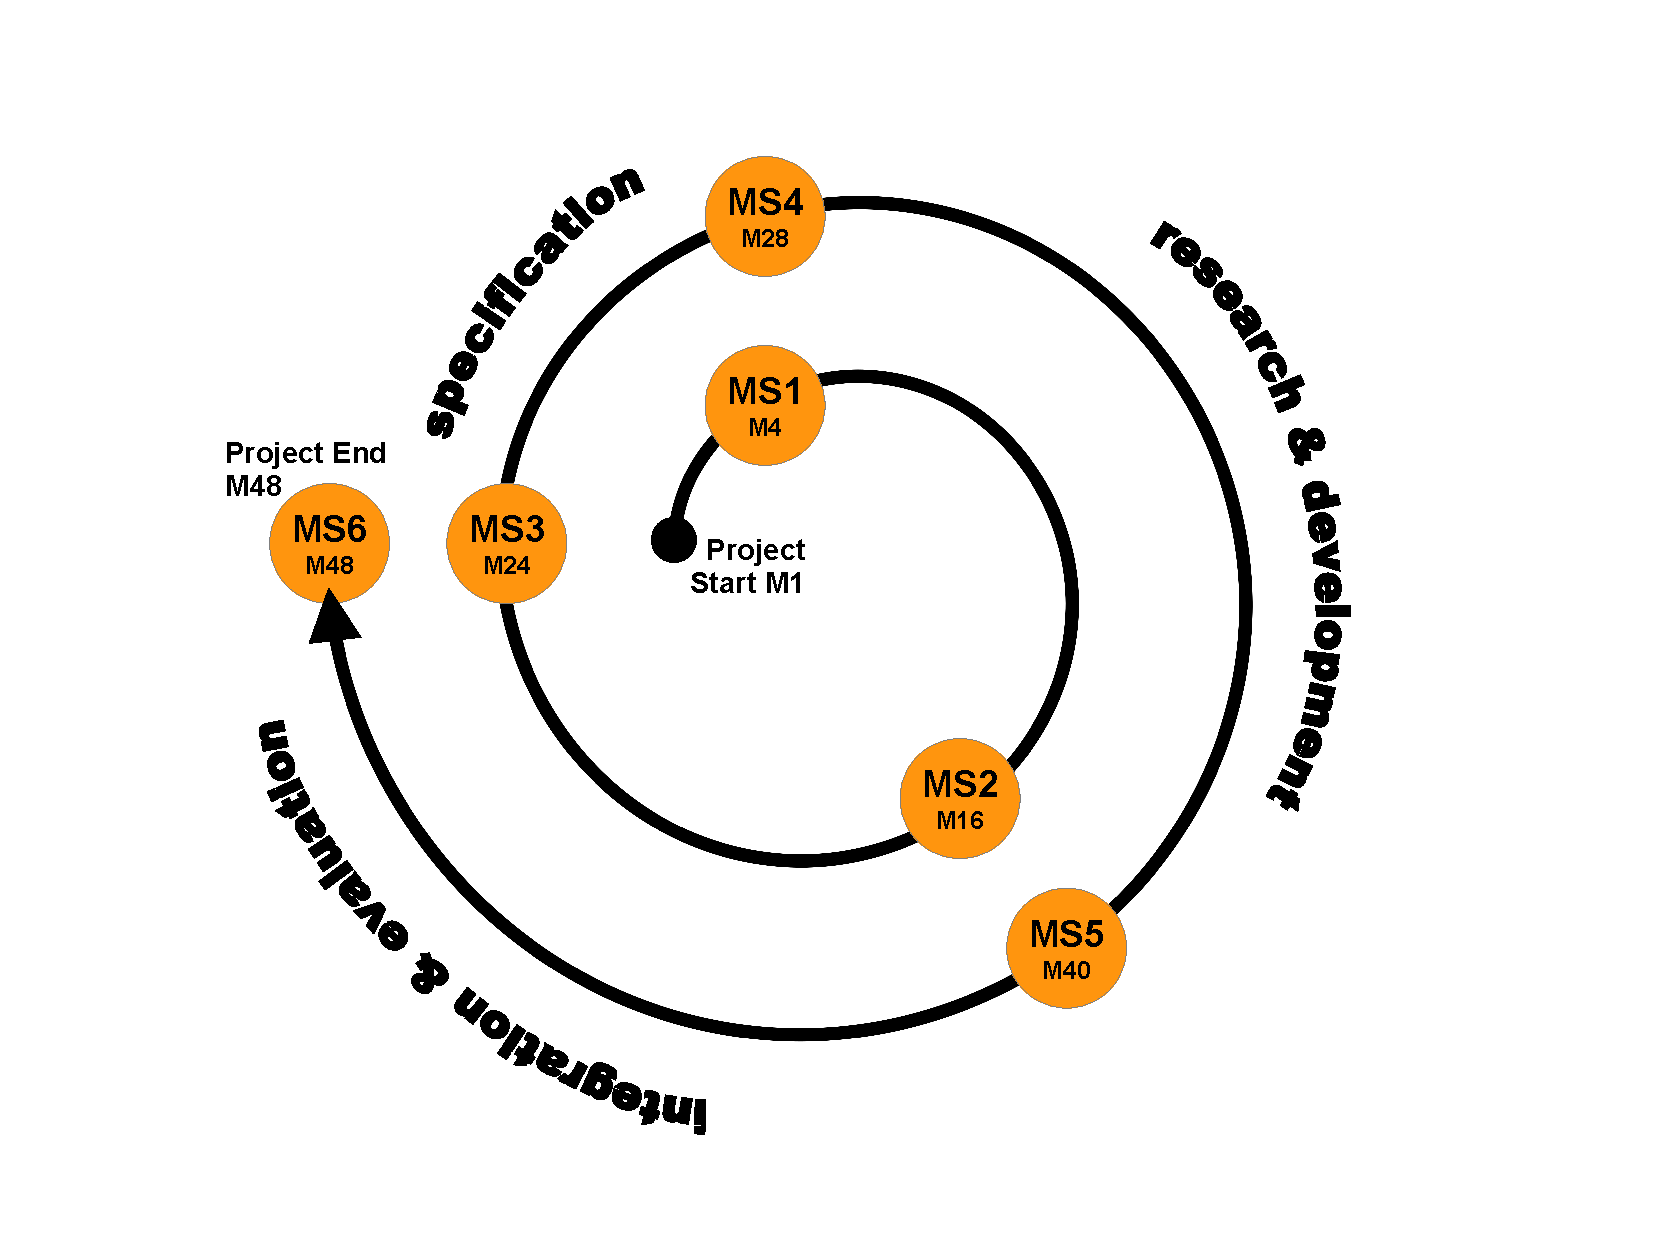
\includegraphics[width=0.6\textwidth]{pics/spiralOverview.pdf}
   \caption{Spiral life-cycle model used in \Project}
\end{wrapfigure}
   \label{fig:spiral}

This model was very successfully applied in previous EC-funded projects by members of the consortium. Using this model for our new endeavor \Project{} will allow us to test and evaluate new developments at early stages.  The spiral development model has the further advantage that it is a risk-reduction oriented model that breaks a project up into smaller projects, the cycles. This allows for improving specifications as experience is gained, and for providing feedback from trials early on in the project.  In the case of \Project, the spiral development model incorporates an intermediate trials/validation phase by the end of the first cycle, which is immediately followed by a re-specification phase (first phase of second cycle). Depending on the results of the intermediate test and validation, the Consortium will refine functional and technical specifications -- and also plan for specific actions that need to be executed in order to mitigate risks.  Within \Project{} risks are taken seriously and are specified for each work package individually. This risk analysis is continuously carried out during the whole project to react to risks as they emerge and minimize their impact on the project.

\paragraph{\textbf{Partner Interaction}}

 The consortium has been primarily assembled according to the individual members' leading expertise in the complementary domains required for successfully completing the bold aims of \Project. However, equally important for the project's success, the consortium members also spot a substantial record of successful previous collaboration (see Section~\ref{sec:consortium})-- thereby reducing interaction-related project risks substantially. To this end, and as has been proven to be successful in the past, integration efforts will commence very early in the project in alignment with the modular approach proposed above.

Although the work is separated into work packages to create efficient interfaces, as described below, all partners will closely collaborate from the onset at and across these interfaces. Meetings between the participants, as well as four consortium-wide integration and testing weeks, for which all partners meet to boost the integration of the individual components, will be carried out during the project at months M17, M24, M41 and M48. The second and fourth of these meetings will coincide with the intermediate and final project evaluation, respectively. In between physical meetings, there will be frequent exchange via telephone, email, a common repository for developments, and web-based services such as forums or status report pages. All of these will serve to boost the integration of our work, to identify problems early on and to measure the progress of the project. We are convinced that a proper joint integration is key in large-scale robotics projects with a significant degree of autonomous behavior, especially if the robots operate in challenging and complex environments as the ones addressed in this project. 

%\begin{figure}[ht]
%\centering
%\subfigure[Spiral life-cycle model used in \Project]{
%   \includegraphics[width=0.45\textwidth]{pics/spiral.jpg}
%   \label{fig:spiral}
% }
% \subfigure[Work Package Overview with key interfaces between the individual work packages.]{
%   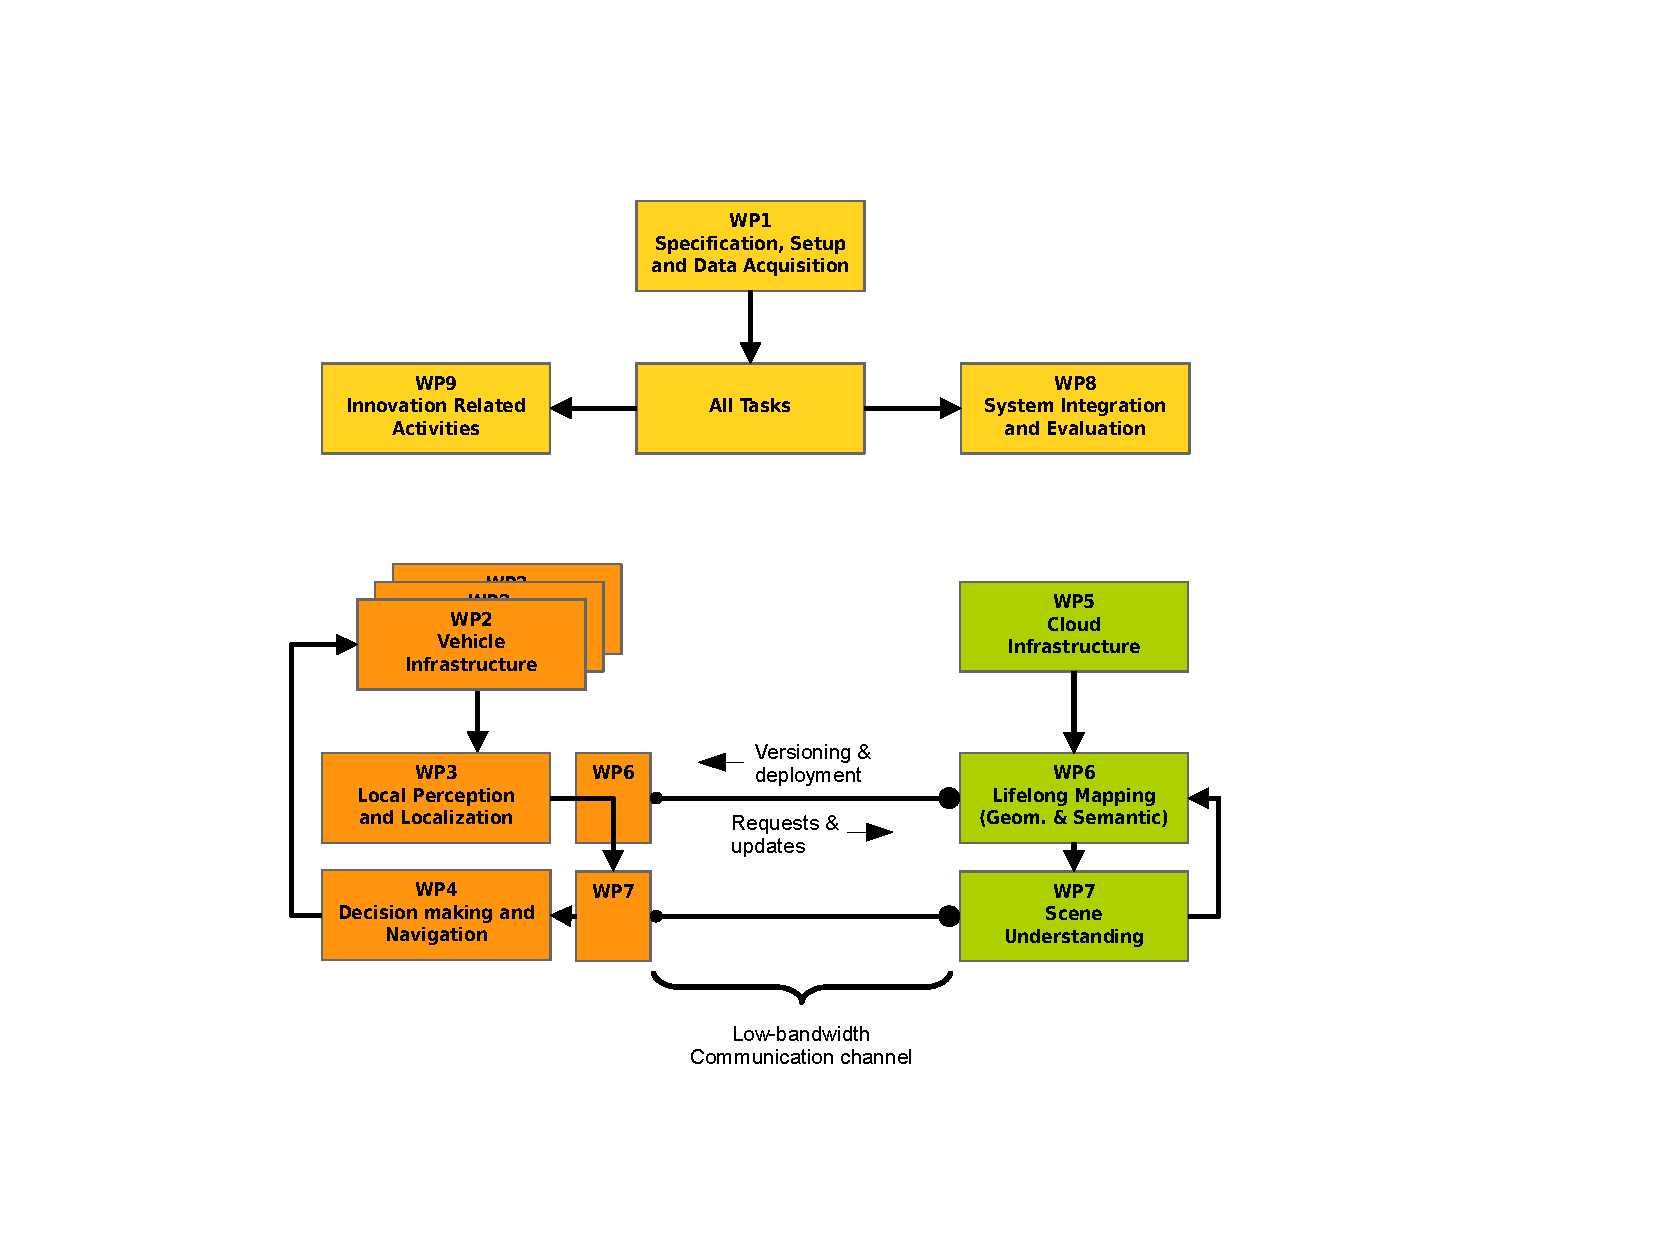
\includegraphics[width=0.45\textwidth] {pics/wpOverview.jpg}
%   \label{fig:wpOverview}
% }
%\label{fig:xxxx}
%\caption{Spiral life cycle model and associated work packages. \todo{\IBM: redo}}
%\end{figure}

\begin{figure}[ht]
  \centering
   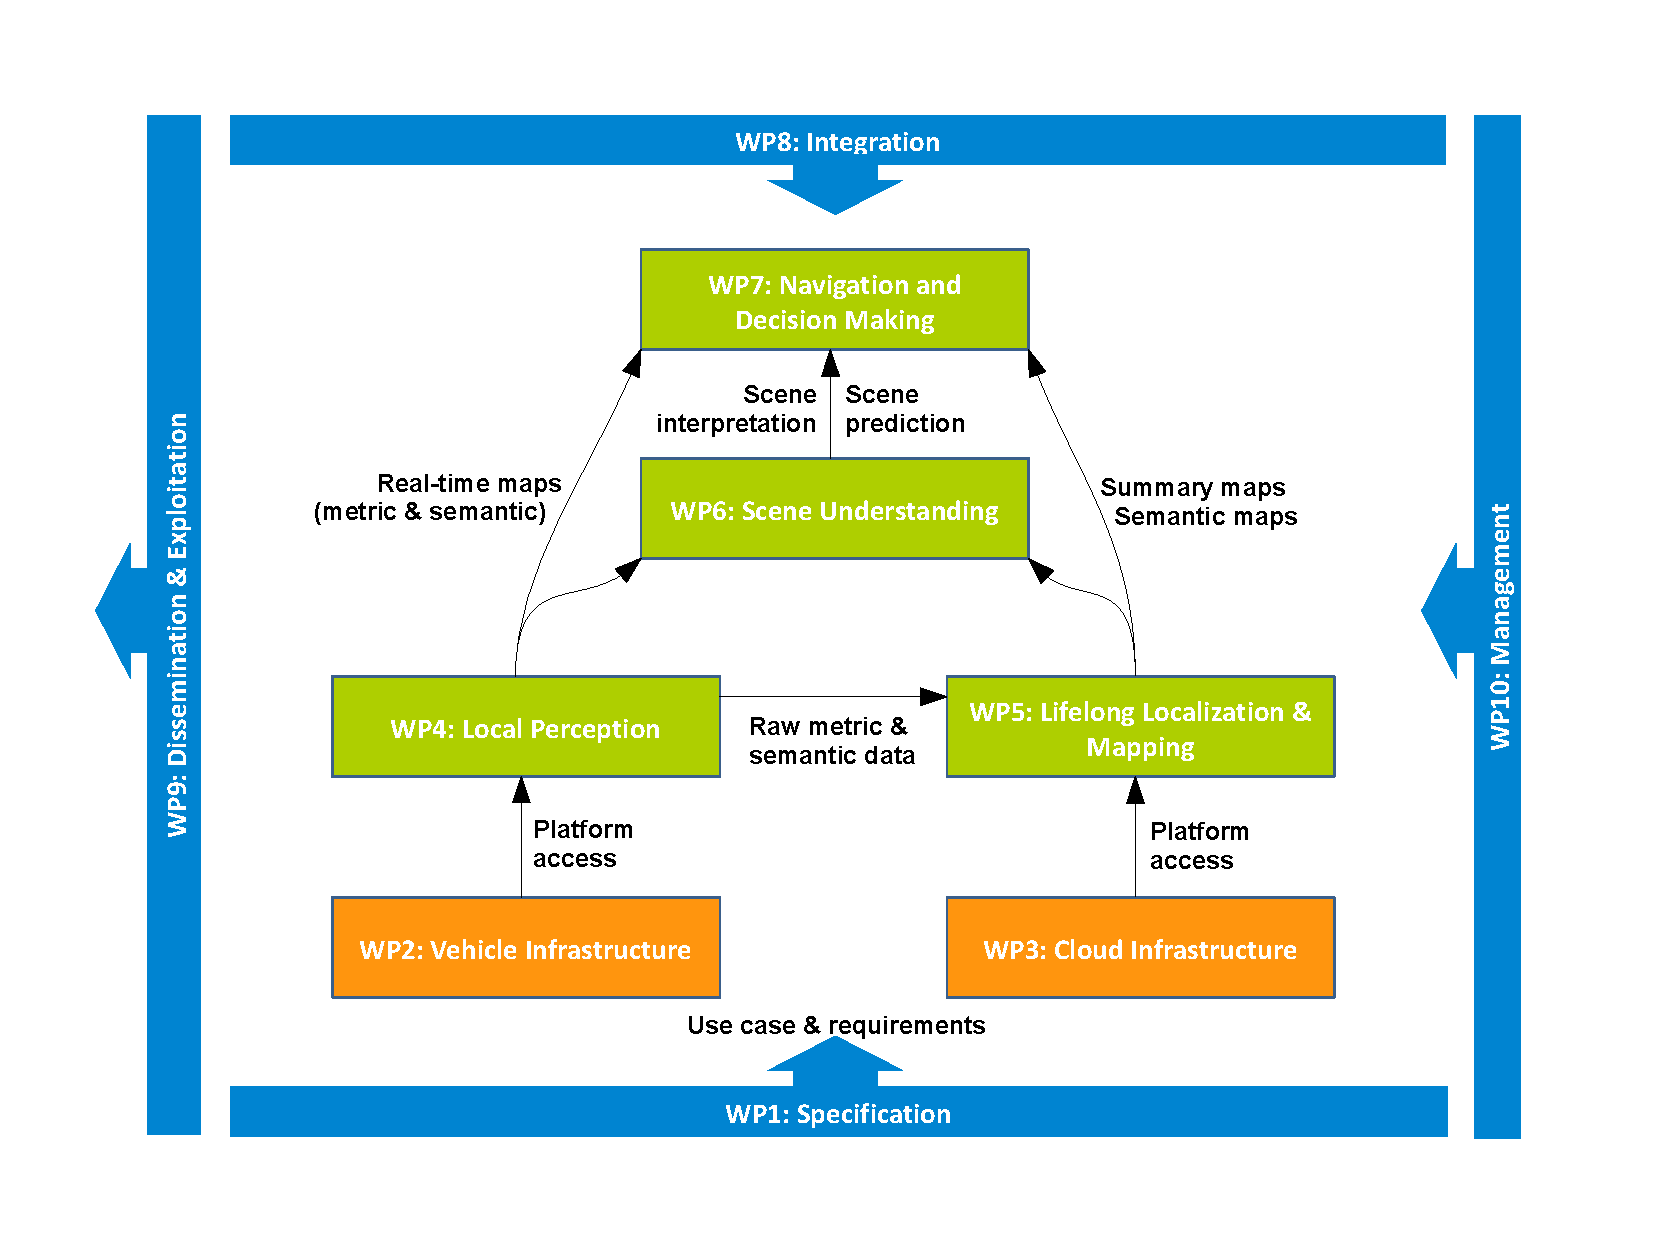
\includegraphics[width=0.8\textwidth] {pics/wpOverviewV2.pdf}
   \caption{Work Package overview with key interfaces between the individual work packages.}
   \label{fig:wpOverview}
\end{figure}



\subsubsection{Detailed Implementation Plan and Work Package Overview}
\label{sec:implementationplan}

The development \& implementation plan of \Project{} follows a logical partition of the work based on the applications addressed within the project. It separates key problems into individual work packages and entrusts their coordination to the consortium partner with the strongest expertise in that area. As a result, the work in \Project{} is  structured into the six technical work packages (WP2 -- WP7) each corresponding to a different key technical or scientific topic that will be addressed, one work package each for the Use Case \& Requirements Specification (WP1), and System Integration \& Evaluation (WP8), respectively -- in alignment with the spiral life cycle model employed. Finally, the project maintains a work package covering important innovation-related activities including dissemination and exploitation (\WPInnovation), and a work package covering aspects related to project management (\WPManagement). Table~\ref{wpleadertab} provides an overview.

\label{wpleadertab}
\begin{center}
{\small
  \begin{tabular}[h]{|c|l|l|}\hline
    {\highlightCell WP} & {\highlightCell Addressed Project Part} & {\highlightCell WP Leader} \\\hline\hline
    \WPSpecificationNo &   \WPSpecificationTitle & \CLUJ \\
    \WPVehicleNo &  \WPVehicleTitle  & \VW \\
    \WPCloudNo & \WPCloudTitle & \IBM \\
    \WPPerceptionNo & \WPPerceptionTitle & \CLUJ \\
    \WPMappingNo & \WPMappingTitle & \ETHZ \\
    \WPSceneUnderstandingNo & \WPSceneUnderstandingTitle & \PRAGUE \\
    \WPNavigationNo & \WPNavigationTitle & \VW \\
    \WPIntegrationNo & \WPIntegrationTitle & \VW \\
    \WPInnovationNo & \WPInnovationTitle & \IBM \\
    \WPManagementNo & \WPManagementTitle & \VW\\
    \hline
  \end{tabular}
}
\end{center}

Each work package is in turn split into several tasks to provide a more detailed structure including an assignment of responsibilities to the individual partners. A detailed description of the work packages, including the connection to other WPs, the personnel resources, tasks, as well as the resulting deliverables is the topic of the remainder of this section.

Before explaining the work packages and involved task in detail starting on Page~\pageref{wp1}, however, we briefly summarize the key topics addressed in the work packages and their inter-dependencies. Please also refer to  Table~\ref{tab:wpoverview} on Page~\pageref{tab:wpoverview} as a  quick reference for the tasks in the work packages and Figure~2 on Page~\pageref{fig:wpOverview} for a chart illustrating the connections between work packages. 



%%%%%%%%%%%%%%%%%%%%%%%%%%%%%%%%%%%%%%%
\paragraph{\textbf{\WPSpecification: \WPSpecificationTitle}} 
This work package targets the overall application-specific challenges of the project and together with \WPIntegration \space enables system-wide considerations within the spiral life-cycle model adopted in \Project (see Figure~\ref{fig:spiral} on Page~\pageref{fig:spiral}). In particular, end user needs and requirements are analyzed with respect to the proposed applications -- which in turn lead to a concretized application specification. Based on these requirements, the structural and functional architectures of the system and components will be specified. During the project duration two cycles of specification and re-specification are performed.


%%%%%%%%%%%%%%%%%%%%%%%%%%%%%%%%%%%%%%%
\paragraph{\textbf{\WPVehicle: \WPVehicleTitle}}
The goal of this work package is to provide fully operational automated vehicles serving the project as data collection platforms, for the test and evaluation of the  perception, localization and mapping, scene interpretation and actuation functionality developed in work packages 4--7, as well as for the demonstration of the overall applications. A fully operational platform will be made available quickly to accelerate research by refurbishing a vehicle from the V-Charge project. Specifications from \WPSpecification will be addressed completely by designing an additional vehicle within the \Project{} project -- available by the second project half. The work package covers the following aspects:
\begin{denseItemize}
\item \textbf{Vehicle buildup} including sensor system, computer system, communication system (in-vehicle as well as between vehicles) as well as HMI elements
\item \textbf{Enabling automated operation} through actuation of all relevant vehicle systems: gas, brakes, steering wheel, gearbox, parking brake, etc.
\item Design and implementation of a framework for \textbf{low-level data acquisition, processing \& communication}
\item\textbf{Calibration and data integrity validation} of the sensor system
\item Installation and integration of \textbf{reference sensors for ground-truth measurements}
\item \textbf{Vehicle maintenance and updates}
\end{denseItemize}


%%%%%%%%%%%%%%%%%%%%%%%%%%%%%%%%%%%%%%%
\paragraph{\textbf{\WPCloud: \WPCloudTitle}}
In this work package a project-wide foundational layer for cloud infrastructure is designed and implemented, allowing for the development, deployment, testing, and operation of the software developed in \Project. This infrastructure consists of a foundational hardware stack and a software stack for managing development, deployment, operation, and long-term data storage. Key activities in \WPCloud include:
\begin{denseItemize}
\item Setup of \textbf{project-wide development infrastructure}. In order to enable collaborative system development state-of-the-art tools will be installed and made accessible to all partners. These include software repository, wiki, issue tracking system, test data server.
\item \textbf{Server hardware specification and setup}. The hardware stack will consist of compute nodes, accelerators, memory, storage
  and communication infrastructure, and will be scoped based on the functional
  and application requirements derived in \WPSpecification.
\item Design of a \textbf{development and deployment tool chain} consisting of a configuration management system and a continuous integration system.
\item Setup of a \textbf{cross-device communication framework} ensuring messaging between applications in the software stacks on the vehicles
  and on the server.
\item Setup and implementation of the \textbf{bulk data storage service} consisting of an object store such as OpenStack Swift, which is ideal for storing unstructured data that can grow without bound. Data storage will be built for scale and optimized for durability, availability, and concurrency across the entire stored data set.
\end{denseItemize}

%In this work package a project-wide foundational layer for the compilation, testing, deployment and operation of project functionality as well as the storage, processing, maintenance and sharing of data across devices is implemented. The framework spans hardware and software infrastructure stacks on the cars as well as on a dedicated server. It exposes a common front-end allowing the same applications (i.e., mapping, localization and scene understanding functionality) to operate on either stack -- with the sole difference being the amount but not the type of resources (compute, memory, storage, data) available to them. Activities in \WPCloud include:
%\begin{denseItemize}
%\item \textbf{Hardware stack}. The hardware stack will be formed by distinct vehicle and server side setups of compute nodes, accelerators, and memory \& storage. The compute nodes are built around IBM POWER processors, building on the OpenPOWER ecosystem. These will be complemented by state-of-the-art commercial FPGA and GPU compute accelerators. Concerning memory, we will provision significant amounts (\todo{How much?}) of standard dynamic random-access (DRAM) memory in combination with non-volatile memory technologies (\todo{RAMDISK?}). This allows the handling and manipulation of significant chunks of the knowledge graph in memory -- thereby practically enabling the large-scale map maintenance and scene understanding applications covered in \Project{}. 
%
%\item \textbf{Software\,/\,virtualization\,/\,runtime\,/\,deployment stack}. The software stack consists of a deployment toolchain, allowing to specify entire deployment stack (OS, system libraries, databases) and dependencies (data type subscriptions, what to do if dependencies change)  in a proper language. It further provides functionality for automatic compilation and testing of committed software, as well as its deployment. \todo{The idea is that each functionality can specify its own operating system, etc. Everything is virtualized and many such instances may run on the same hardware. Communication is via message passing over TCP (e.g., via MQTT). Furthermore, we need to ensure that each of the virtual machines has access to some joint storage DBs, such as the map. The map DB and maintenance could again be specified as a virtual machine... }. \todo{A runtime scheduler will be part of each virtual machine, and will execute the programs based on scripted events and conditions}. \todo{Deployment will be specified from a separate serer instance (e.g., where the overall code will be maintained), and can be scripted such that entire stacks and stack dependencies are deployed to the server and the vehicles. Prior to deployment we will provide functionality for automated compilation, testing of code based on predefined rules (i.e., once every x duration, or once dependencies have changed). Web-based access control and commit control}. \todo{We need to deploy a yellow-zone server!!}.
%
%\item \textbf{Messaging}. Communication between vehicles and the server and, indeed, between the various virtual machines on every hardware stack will be implemented based on the publish-subscribe principle. We intend to use the the open source Message Queue Telemetry Transport (MQTT) standard originally developed at IBM to this end. It features precise access control, data encryption, small overhead communication important for wireless operation, and various forms of Quality of Service (QoS)  settings.
%
%\item \textbf{Data representation \& curation}. It is extremely important that data is represented consistently over the entire project, that it is efficiently accessible by all technical functionality, and that it is curated between the vehicles and the server. Tasks include knowledge representation and storage. This will be done as a knowledge graph, unifying metric and semantic maps of WPxx and semantic extractions of WP3, and providing a single interface for scene interpretation (WP7). Particular focus will be laid on the propoer data structures and storage location for each of the data sources. Other tasks include data curation, hence the adding, deleting, merging -> essentially versioning) consistent representation across devices, dependency handling. We will begin with a centralized approach orchestrated from the server, and will then also consider more decentralized options.
%\end{denseItemize}


%%%%%%%%%%%%%%%%%%%%%%%%%%%%%%%%%%%%%%%
\paragraph{\textbf{\WPPerception: \WPPerceptionTitle}}
This work package provides the vehicle-side online sensing functionality required for automated driving in low-speed urban environments. The work package covers the following primary aspects:
\begin{denseItemize}
\item \textbf{Specification and design of on-board sensing}
\item \textbf{On-board 360\degree \space multi-sensorial perception} based on a set of well selected sensors including laser scanners, radars, large field of view cameras, and stereo cameras disposed in a configuration offering good coverage, redundancy and good measurement accuracy.

\item \textbf{Spatio-temporal and appearance based low-level representation} The low level representation will integrate 3D position, 3D motion and intensity or color components. This will benefit from the fusion of low-level information coming from multi-sensors.

\item \textbf{Refinement of detection, tracking, and classification capabilities and environment sensorial representation}. The intention is to use a spatio-temporal and appearance based low level representation for each pixel, feature or object consisting of 3D position, 3D motion and intensity or color components. This approach will lead to a better detection or clustering of the object or object parts, to a better tracking and classification. Word Channel and Deep Learning methods will be investigated for improving the classification results.
%\item Generation of an environmental model suitable for automated navigation. Compact representation methods will be investigated and developed for environment representation starting from the classified elevation map, stixel representation and 3D voxel representation.
\end{denseItemize}


%%%%%%%%%%%%%%%%%%%%%%%%%%%%%%%%%%%%%%%
\paragraph{\textbf{\WPMapping: \WPMappingTitle}}
This work package develops metric accurate localization and lifelong mapping functionality across vehicles and the server backend. To this end raw sensor as well as semantic data recorded and made available in \WPPerception is collected in a cloud-based mapping backend, where relevant information is extracted and condensed into a compact map representation that can  efficiently be distributed back to the vehicles for localization purposes. The WP can be divided into three key areas:
\begin{denseItemize}
\item \textbf{Online Localization and Mapping} This task employs real-time online localization algorithms on the vehicles. Locally relevant map segments are requested from the mapping backend. Local sensor data is then matched against the map to be able to estimate the vehicle's pose in the map. To guarantee uninterrupted localization availability under all conditions, novel ways to deal with lighting, weather and seasonal change have to be investigated. Research in this area involves striving for performance wrt. metric accuracy, speed and data transmission rates, as well as increasing robustness to appearance change and developing new and efficient ways to feed sensor data back to the mapping backend.
\item \textbf{Map Maintenance and Summarization}. The mapping backend collects sensor data from various agents over long-term operations. Algorithms to assess data accuracy and trustworthiness, to handle structural change as well as encode different appearances are necessary to allow long-term localization in changing environments. It is the scope of this task to collect, assess, register and filter incoming data and to produce compact generic representations ('summary-maps') encoding the most useful information for localization independent of the current environmental conditions. These summary-maps can then be fed back on request to the agents for efficient localization purposes.
\item \textbf{Semantic Information Integration}. The map described above will serve as a backbone for all kinds of higher level semantic information to be represented in. While collecting, classifying and representing this semantic information is done within the scope of \WPPerception and \WPSceneUnderstanding, the map backend enables integration, managing and versioning of the semantic information.
\end{denseItemize}


%The goal of this WP is to provide metrically accurate localization at all times. For this, a map of the agent's environment is recorded, managed and curated.
%The map contains enough information to allow metrically accurate localization across all possible environments, weather and lighting conditions, including night-time.
%Raw sensor data from various agents is collected in a cloud-based mapping backend, where relevant information is extracted and condensed into a compact map representation that can  efficiently be distributed back to the agents for localization purposes. This forms a closed-loop cycle between a fleet of agents and the mapping backend infrastructure.
%In this way, the map is continuously updated and maintained respecting both appearance and structural change on short-term to long-term time scales.
%It further  provides geometrically consistent coordinate frames in which higher level semantic information can be registered.
%\begin{figure}[H]
%\begin{center}
%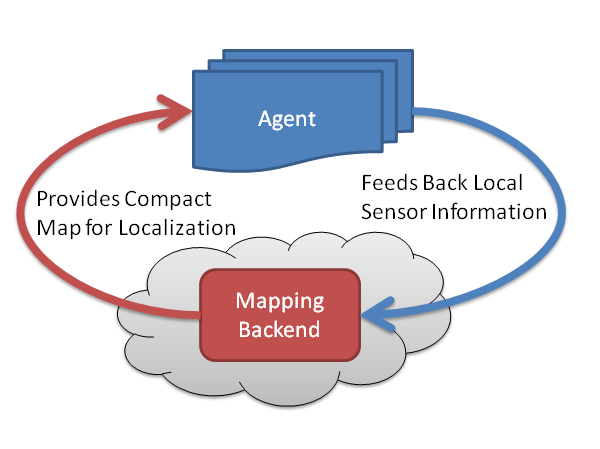
\includegraphics[width=0.5\textwidth]{pics/localization_feedback_loop.png}
%\caption{Feedback-Loop Between Multi-Agent Localization and the Cloud-Based Mapping Backend.}
%\label{fig:pert}
%\end{center}
%\end{figure}
%
%The WP can be divided into four main sub-tasks as follows:
%\begin{denseItemize}
%\item \textbf{Online Localization} This task employs real-time online localization algorithms on the agents. Locally relevant map segments are requested form the mapping backend. Local sensor data is then matched against the map to be able to estimate the agent's pose in the map. Research in this area involves striving for performance wrt. metric accuracy, speed and data transmission rates, as well as developing new and efficient ways to feed sensor data back to the mapping backend.
%
%\item \textbf{Apperance-Based Localization and Mapping}. Accurate and uninterrupted localization around the clock, across seasons and varying weather conditions forms a key requirement for all tasks involved in this project. In order to achieve this goal, identifying the current environmental condition and using this information to infer what sensor data is likely to appear in the imminent future is key and the scope of this task. It shall also allow formulating specific appearance related requests to the mapping backend depending on the current environment condition the agent is perceiving.
%
%\item \textbf{Map Maintenance and Summarization}. The mapping backend collects sensor data from various agents over long-term operations. Algorithms to assess data accuracy and trustworthiness, to handle structural change as well as encode different appearances are necessary to allow long-term localization in changing environments. It is the scope of this task to collect, assess, register and filter incoming data and to produce compact generic representations ('summary-maps') encoding the most useful information for localization independent of the current environmental conditions. These summary-maps can then be fed back on request to the agents for efficient localization purposes.
%
%\item \textbf{Semantic Information Integration}. The map described above will serve as a backbone for all kinds of higher level semantic information to be represented in. While collecting, classifying and representing this semantic information is done within the scope of WP3 and WP7, the map backend developed in WP6 must allow integrating and managing the semantic information in the mapping backend respectively. This task aims at developing a smooth framework and process for semantic data to be integrated into the mapping backend.
%\end{denseItemize}


%%%%%%%%%%%%%%%%%%%%%%%%%%%%%%%%%%%%%%%
\paragraph{\textbf{\WPSceneUnderstanding: \WPSceneUnderstandingTitle}}
Beside local perception it is important to provide the navigation module of \WPNavigation with a high level assessment of the environment, in order to assist it in selecting the proper driving behavior. This work package targets all aspects contributing to understanding the local scene in the surroundings of the car, including driving mode and behavior of other roads occupants. It will hence explore and develop techniques
\begin{denseItemize}
\item to \textbf{represent the environment in scenarios},
\item to fuse information from various \Project{} sensor sources and derivatives thereof (including digital maps, online raw sensor perception, road users' behavior perception, current location, and further contextual information) to create a \textbf{high level scenario description and interpretation}. Examples of such a high-level interpretation include: other car willing to overtake; other car willing to exit the lane; traffic jam ahead; road work; and entering pedestrian area,
%\item for \textbf{context based road users' behavior analysis}. We will extend the dynamic object tracking techniques developed in \WPPerception by complementing them with visual perception information and high level reasoning, to create a profile of each road user surrounding the ego vehicle.
\item for object motion prediction or \textbf{scene prediction}, which is guided by the high-level scenario/behavior information,
\item for \textbf{self-assessment}. Data from Work Packages 4-6 will be analyzed to identify potential data integrity issues or infer context-dependent system limitations.
\end{denseItemize}


%%%%%%%%%%%%%%%%%%%%%%%%%%%%%%%%%%%%%%%
\paragraph{\textbf{\WPNavigation: \WPNavigationTitle}}
In this work package decision making and navigational abilities necessary for automated operation in urban areas are adapted from previous projects of the consortium members and further developed. This work package relies on information from the online local perception, scene understanding, as well as from offline metric and semantic mapping. The activities within this task range from route and tactical planning, to maneuver and trajectory planning, to trajectory control. The decision making and navigation stack will take into account constraints arising from traffic rules, collision risks, time budget for reaching the target destination, etc. Attention will be also devoted the question of map verification and fall back strategies in case the map turns out to be outdated/erroneous.


%%%%%%%%%%%%%%%%%%%%%%%%%%%%%%%%%%%%%%%
\paragraph{\textbf{\WPIntegration: \WPIntegrationTitle}}

The individual components of \Project{} -- grouped into work packages -- can be developed and evaluated individually to some extent only.  As Figure~\ref{fig:wpOverview} on Page~\pageref{fig:wpOverview} illustrates, information exchange and thus interdependency between the tasks and WPs is substantial. Integration and evaluation at the system level, with a strong focus on the proposed applications, thus becomes critical.

To this end, \WPIntegration will be responsible for the integration and testing of the individual modules, as well as system-wide testing and validation with a special emphasis towards the proposed applications. This includes the organization of the integration and testing weeks and the smooth integration of the technologies developed in this project. Thus, all work packages will strongly interact with \WPIntegration. Activities in \WPIntegration include:
\begin{denseItemize}
%mru: moved to cloud infrastructure WP
%\item \textbf{Development Repository}. All partners will contribute software modules for the integrated system. The versions of all software modules will be handled using a central development repository with access to all partners.
\item \textbf{Integration Plan}. The integration plan will specify which components have to provide certain functionality to allow for a successful integration. It will furthermore contain a detailed time line for the integration and thus serves as a manual for the integration weeks.
\item \textbf{Integration tools and processes}. In order to make the integration and test efficient and effective a set of tools and processes will be installed or developed, including checklists, and developer guidelines.
\item \textbf{System Integration and Testing Weeks}. We will have four integration and testing weeks throughout the project life time and the integration task will start early on so that a first integrated working system becomes available early in the project life-cycle. The four integration and testing weeks will be the key concept to ensure a smooth integration of all the individual modules to a working subsystem. They will bring together the researchers, help to identify problems, and boost the overall development process.
\item \textbf{Evaluation}. A proper evaluation is essential to measure the capabilities of the system, scientific advancement, and  the success of the overall project. This work package thus on one hand addresses the evaluation of the individual components; the measures for success, specified in the individual work packages, will serve as the basis for the evaluation. On the other hand \WPIntegration will measure the performance of the overall integrated system as specified by the application scenarios. Finally scientific progress will be evaluated by the quality and quantity of papers published in journals and relevant conferences. 
\end{denseItemize}


%%%%%%%%%%%%%%%%%%%%%%%%%%%%%%%%%%%%%%%
\paragraph{\textbf{\WPInnovation:  \WPInnovationTitle}}
This work package covers the following aspects:
\begin{denseItemize}
\item \textbf{Dissemination activities}: ensuring the proper dissemination of the \Project{} project and promoting awareness of results in the general, business and scientific community at large. This is envisioned to be in the form of documents, brochures, Web-publications, workshops, articles, papers for journals and conferences or other publicity work. More details on planned dissemination activities can be found on Page~\pageref{sec:diss}.
\item \textbf{Exploitation plan} ensuring the proper exploitation of the \Project{} results. This includes activities such as an address database of related stakeholders, potential customers, interested individuals and companies, and the identification and pursuing of exploitable results. More information on exploitation activities can be found on Page~\pageref{sec:expl}.
\item \textbf{Management of Knowledge including IPR handling}. This will include an internal collaboration environment in addition to the public website, and data management ensuring that data produced by the project is available for further research -- while respecting the data policies of the consortium members. In addition this aspect ensures IPRs are properly handled and patents are filed where and when necessary. More detail on the planned management of knowledge and IPR handling can be found on Page~\pageref{sec:iprhandling}.
\end{denseItemize}


%%%%%%%%%%%%%%%%%%%%%%%%%%%%%%%%%%%%%%%
\paragraph{\textbf{\WPManagement: \WPManagementTitle}}
The \Project{} project management structure is characterized by the following formal roles: (i) Project Coordinator and Steering Committee; and (ii) Work package leaders. In terms of formal process, the work package leaders will be responsible for the planning, scientific management and progress of their work package and will have to report the progress to the project coordination team consisting of the Project Coordinator \Coordinator{}. The work package leaders' responsibility is further to identify and highlight problems as early as possible. This approach ensures a task-driven scientific management while maintaining effective overall control by the coordination team.  For the day-to-day work on the project, virtual project teams are formed according to the involved participants in the individual tasks. The Steering Committee -- formed by representative from each partner -- serves as the main forum for decisions and the responsible instance to resolve disputes. Decisions will require majority and will be binding. Besides the formal channels described above, communication will also be performed on a non-periodic basis for the exchange of unstructured information as well as the rapid clarification of details, etc. In this way, the consortium will effectively track the progress of project activities while, at the same time, it will keep the administration overhead at a low level. A more detailed account of the \Project{} project management structure is provided in Section~\ref{sec:management} starting on Page~\pageref{sec:management}.


